\chapter{Proposta}

Conforme apresentado nos capítulos anteriores, a modelagem de um sistema de detecção de fraude com a utilização de técnicas inspiradas no sistema imunológico natural busca trazer diversas vantagens tanto no processo de planejamento quanto na sua arquitetura final. Esse trabalho busca identificar exatamente \emph{quanto} esses modelos podem aperfeiçoar os métodos existentes. O método utilizado é a comparação dos resultados da classificação de algoritmos tradicionais e Sistemas Imunológicos Artificiais sobre um mesmo conjunto de dados. Esta seção apresenta os elementos principais para o desenvolvimento da proposta.

\section{Comparação dos algoritmos}

A comparação do desempenho de diferentes algoritmos deve ser baseada em critérios sólidos para que tenha algum valor prático. Assim, nesse trabalho, a comparação dos algoritmos foi divida em duas etapas: execução e análise.

A etapa de execução consiste em executar os algoritmos utilizando \emph{grid search} e \emph{cross-validation}. Utilizar \emph{cross-validation} diminui a influência do conjunto de dados no resultado dos testes. Como o algoritmo é treinado e testado várias vezes, cada vez com uma divisão diferente do conjunto de dados para treinamento e testes, quaisquer tendências nos dados são eliminadas, e o resultado se torna mais confiável.

Geralmente, o \emph{grid search} é utilizado para selecionar os melhores parâmetros para um modelo, para que esses parâmetros sejam incorporados no sistema final, obtendo a melhor performance possível. Nesse trabalho, ele será utilizado para gerar o melhor modelo possível para cada algoritmo, para que eles possam ser comparados igualmente. Em resumo, a etapa de execução consiste em:

\begin{enumerate}
    \item Para cada algoritmo:
        \begin{enumerate}
            \item Utilizar \emph{grid search} para otimizar os parâmetros para os dados.
            \item Utilizando esses parâmetros, executar os testes usando \emph{cross-validation}.
        \end{enumerate}
\end{enumerate}

Durante a etapa de execução, serão coletados dados sobre os resultados dos testes. Esses dados serão utilizados na etapa de análise, gerando, por fim, a comparação. Esses critérios foram selecionados de acordo com a análise de trabalhos recentes e relevantes nas áreas de mineração de dados e detecção de fraude. Em resumo, a etapa de análise consiste em::

\begin{enumerate}
    \item Calcular, para o resultado de cada algoritmo:
        \begin{enumerate}
            \item O erro médio relativo.
            \item O índice de Youden.
            \item O índice de Youden com significância maior para os falsos negativos.
        \end{enumerate}
\end{enumerate}

O erro médio relativo é uma medida padrão simples, que mostra o quanto o resultado de um teste difere dos valores corretos. Ele é utilizado como uma métrica simples para o desempenho de um algoritmo, e pode ser utilizado como análise superficial na comparação de algoritmos. No entanto, o erro médio relativo não pode ser utilizado como métrica única: devido a simplicidade do seu cálculo, não é suficiente para a análise de áreas mais complexas como a detecção de fraude.

O índice de Youden é uma medida de performance que leva em consideração não só o número de instâncias classificadas corretamente. Para que o índice de Youden seja alto, tanto a taxa de falsos positivos quanto a de falsos negativos deve ser baixa. Conforme apresentado na seção \ref{sec:eval_fraud}, na detecção de fraude os falsos positivos são muito mais críticos do que os falsos positivos. Assim, serão calculados dois índices: o índice de Youden padrão e o índice de Youden com maior significância para os falsos negativos. Esse é calculado através da fórmula:

\begin{equation}
    \vspace{2mm}
    J = 0.25 * sensibilidade + 0.75 * especificidade
    \vspace{2mm}
\end{equation}

Conforme o padrão nesse tipo de experimento, os dados serão apresentados em formato de tabela e gráfico. Os critérios escolhidos já são parte integrante dos resultados exibidos na execução do WEKA. Essa escolha reflete tanto a aderência dessa plataforma aos padrões da área como a facilidade que uma ferramenta desse tipo oferece na determinação do método de avaliação.

\iffalse

\section{Mineração de dados}

Introdução à mineração.
Etapas (figura).
Dados.
Pré-processamento.

\section{Critérios}

Critérios que serão utilizados para a comparação e justificativa.

\section{WEKA}

ALgoritmos inspirados no sistema imunológico que serão utilizados.

\subsection{CLONALG}
\subsection{AIRS}
\subsection{Immunos}
\fi

\section{Descrição dos dados}

Para os testes foram utilizados dois conjuntos de dados contendo informações de contas de cartões de crédito. Esses dados estão disponíveis publicamente e fazem parte de um projeto chamado StatLog \cite{Michie1994}. Esse projeto foi concebido para testar diversos métodos de classificação em problemas grandes e comercialmente relevantes, comparando os seus resultados e determinando o quanto eles atendiam as necessidades da indústria. Conforme a sua própria descrição, os objetivos do projeto eram três:

\begin{enumerate}[a)]
    \item Possibilitar medidas críticas de desempenho para procedimentos de classificação disponíveis,
    \item Indicar a natureza e escopo dos desenvolvimentos futuros necessários para que os métodos atendam as necessidades e expectativas dos usuários e
    \item Indicar as direções mais promissoras de desenvolvimento para abordagens comercialmente imaturas.
\end{enumerate}

Os conjuntos de dados são denominados German Credit (Cr.Ger) e Australian Credit (Cr.Aust). Ambos contém informações sobre contas de crédito, conforme apresentado nas próximas seções.

\subsection{Cr.Ger}

Esse conjunto de dados foi cedido pelo professor Hans Hoffman, da Universidade de Hamburgo. Os atributos e valores que esses atributos podem assumir são descritos na listagem \ref{lst:ge_dataset} (traduzido do original)\footnote{Na descrição dos atributos, DM significa \emph{deutsche mark} (marco alemão), a moeda corrente na Alemanha na época da coleta dos dados. Para efeito de comparação, o Banco Central Europeu estipulou a conversão irrevogável do marco alemão, a partir de 1º de janeiro de 1999, em DM 1.95583 = \euro 1 (http://www.ecb.int/press/pr/date/1998/html/pr981231$\textunderscore$2.en.html).}.

\vspace{1cm}
\begin{lstlisting}[caption=Atributos do conjunto de dados alemão,label=lst:ge_dataset]
    Atributo 1: (qualitativo)
    Situação da conta corrente existente
    A11 : ... < 0 DM
    A12 : 0 <= ... < 200 DM
    A13 : ... >= 200 DM
    A14 : sem conta corrente

    Atributo 2: (numérico)
    Duração em meses

    Atributo 3: (qualitativo)
    Histórico de crédito
    A30 : nenhum crédito retirado / todos os créditos pagos apropriadamente
    A31 : todos os créditos nesse banco pagos apropriadamente
    A32 : créditos existentes pagos apropriadamente até agora
    A33 : atraso no pagamento no passado
    A34 : conta crítica / outros créditos existentes (não nesse banco)

    Atributo 4: (qualitativo)
    Propósito
    A40 : carro (novo)
    A41 : carro (usado)
    A42 : móveis/equipamento
    A43 : rádio/televisão
    A44 : eletrodomésico
    A45 : reparos
    A46 : educação
    A47 : (férias - não existe no conjunto de dados)
    A48 : reciclagem profissional
    A49 : negócios
    A410 : outros

    Atributo 5: (numérico)
    Quantidade de crédito

    Atributo 6: (qualitativo)
    Poupança
    A61 : ... < 100 DM
    A62 : 100 <= ... < 500 DM
    A63 : 500 <= ... < 1000 DM
    A64 : .. >= 1000 DM
    A65 : desconhecido / sem poupança

    Atributo 7: (qualitativo)
    Emprego atual desde
    A71 : desempregado
    A72 : ... < 1 ano
    A73 : 1 <= ... < 4 anos
    A74 : 4 <= ... < 7 anos
    A75 : .. >= 7 anos

    Atributo 8: (numérico)
    Taxa de parcelamento em porcentagem do rendimento disponível

    Atributo 9: (qualitativo)
    Estado civil e sexo
    A91 : masculino : divorciado/separado
    A92 : feminino : divorciada/separada/casada
    A93 : masculino : solteiro
    A94 : masculino : casado/viúvo
    A95 : feminino : solteira

    Atributo 10: (qualitativo)
    Outros devedores / fiadores
    A101 : nenhum
    A102 : devedor solidário
    A103 : fiador

    Atributo 11: (numérico)
    Residência atual desde

    Atributo 12: (qualitativo)
    Propriedade
    A121 : imóvel
    A122 : se não A121 : financiamento / seguro de vida
    A123 : se não A121/A122 : carro ou outro, não incluso no atributo 6
    A124 : desconhecido / sem propriedade

    Atributo 13: (numérico)
    Idade em anos

    Atributo 14: (qualitativo)
    Outros planos de parcelamento
    A141 : banco
    A142 : lojas
    A143 : nenhum

    Atributo 15: (qualitativo)
    Residência
    A151 : alugada
    A152 : própria
    A153 : gratuita

    Atributo 16: (numérico)
    Número de créditos existentes nesse banco

    Atributo 17: (qualitativo)
    Emprego
    A171 : desempregado / sem proficiência / não-doméstico
    A172 : sem proficiência / doméstico
    A173 : proficiente / funcionário público
    A174 : administrador / auto-empregado /
           empregado altamente qualificado / oficial

    Atributo 18: (numérico)
    Número de dependentes

    Atributo 19: (qualitativo)
    Telefone
    A191 : nenhum
    A192 : sim, registrado sob o nom do consumidor

    Atributo 20: (qualitativo)
    Trabalhador estrangeiro
    A201 : sim
    A202 : não
\end{lstlisting}

\subsection{Cr.Aust}

Os atributos do conjunto de dados australiano são descritos na listagem \ref{lst:prop_au_dataset} (traduzido do original). Uma grande desvantagem, muito comum nesse tipo de conjunto de dados (seção \ref{sec:fraud_data}), é a de o nome dos campos ter sido alterado, perdendo o significado original. Para garantir a privacidade das informações contidas no conjunto de dados, provavelmente por questões competitivas, a empresa que cedeu os dados utilizou um processo de anonimização, garantindo que as informações confidenciais não possam ser recuperadas.

Os dados ainda podem ser utilizados para a validação de sistemas de detecção, mas não é possível saber de que forma o sistema chegou ao diagnóstico, tornando o resultado bem menos útil.

\vspace{1cm}
\begin{lstlisting}[caption=Atributos do conjunto de dados Cr.Aust, label=lst:prop_au_dataset]
A1: b, a
A2: contínuo
A3: contínuo
A4: u, y, l, t
A5: g, p, gg
A6: c, d, cc, i, j, k, m, r, q, w, x, e, aa, ff
A7: v, h, bb, j, n, z, dd, ff, o
A8: contínuo
A9: t, f
A10: t, f
A11: contínuo
A12: t, f
A13: g, p, s
A14: contínuo
A15: contínuo
A16: +,- (atributo de classe)
\end{lstlisting}

\section{Algoritmos}

Os algoritmos que serão utilizados para a comparação são um pacote de algoritmos desenvolvido por Jason Brownlee \cite{Brownlee2011}, na versão mais atual (1.8, maio de 2011). Esse pacote foi especialmente desenvolvido para a plataforma de aprendizagem de máquina WEKA (descrita na seção \ref{sec:prop_weka}) e são disponibilizados através de uma licença aberta (GNU GPL). Nele, são implementados diversas categorias de algoritmos de Redes Neurais e Sistemas Imunológicos Artificiais:

\begin{enumerate}
    \item Redes neurais
    \begin{enumerate}[a)]
        \item \textbf{Learning Vector Quantization (LVQ)}: similar às redes neurais, que utiliza aprendizagem supervisionada, baseada em protótipos, para classificação de dados. É similar ao algoritmo de k-vizinhos mais próximos e um precursor do próximo algoritmo.
        \item \textbf{Self-Organizing Map (SOM)}: algoritmo de redes neurais que utiliza aprendizagem não-supervisionada. Mapeia os valores da base de dados produzindo um mapa: um espaço de duas dimensões, uma representação discreta dos dados de entrada.
        \item \textbf{Feed-Forward Artificial Neural Network (FF-ANN)}: tipo de algoritmo de redes neurais onde o sinal é propagado na direção entrada-saída, sem conexões de \emph{feedback}.
    \end{enumerate}
    \item Sistemas Imunológicos Artificiais
    \begin{enumerate}[a)]
        \item \textbf{Artificial Immune Recognition System (AIRS)}: algoritmo imunológico supervisionado descrito na seção \ref{sec:prop_airs}.
        \item \textbf{Clonal Selection Algorithm (CLONALG)}: um dos principais algoritmos imunológicos, o algoritmo da seleção clonal, descrito na seção \ref{sec:ais_clonalg}.
        \item \textbf{Immunos-81}: algoritmo imunológico descrito na seção \ref{sec:prop_immunos}.
    \end{enumerate}
\end{enumerate}

Desses, os algoritmos de Sistemas Imunológicos Artificiais (2) serão utilizados para comparação com os métodos tradicionais. O algoritmo da seleção clonal (CLONALG) foi descrito na seção \ref{sec:ais_clonalg}. Os outros dois são descritos nas próximas seções. A figura \ref{fig:prop_wekaais} mostra esses algoritmos conforme apresentados na interface do WEKA.

\begin{figure}[h!]
    \centering
    \caption{Algoritmos no WEKA}
    \label{fig:prop_wekaais}
    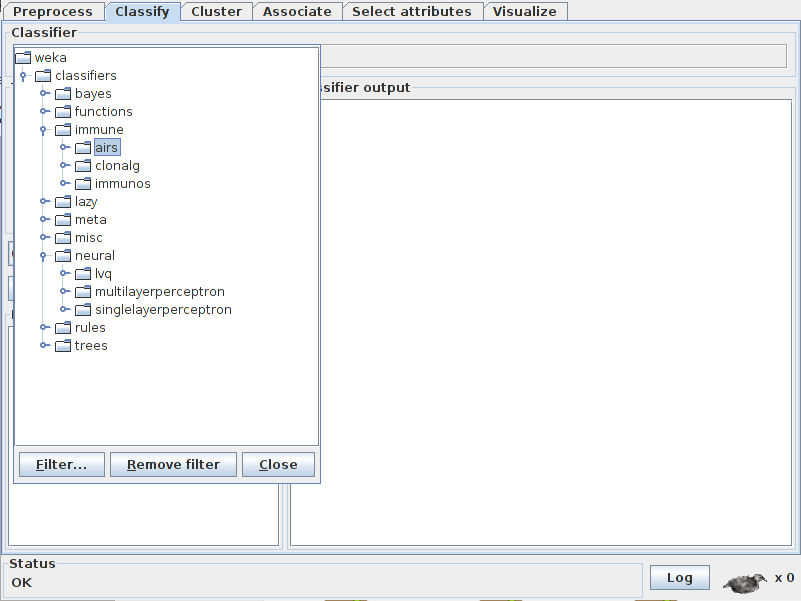
\includegraphics[width=0.75\textwidth]{img/weka_ais.png}
\end{figure}

\subsection{AIRS}
\label{sec:prop_airs}

Esse algoritmo foi criado por Andrew Watkins \cite{Andrew2003} e tinha como objetivo implementar um Sistema Imunológico Artificial que utilizasse aprendizagem supervisionada. Na época de seu desenvolvimento, a área de algoritmos imunológicos supervisionados não havia sido explorada, apesar da pesquisa intensa na área de algoritmos imunológicos não-supervisionados \footnote{De acordo com o autor, o único outro algoritmo imunológico supervisionado era o Immunos, apresentado na próxima seção.}.

Por esse motivo, esse foi o primeiro algoritmo supervisionado a implementar a maior parte das técnicas inspiradas nos sistemas imunológicos, como: modelagem dos dados como antígenos e anticorpos, expansão clonal dos linfócitos, mutação e maturação de afinidade e memória imunológica.

Na definição desse algoritmo também foi aplicado o formalismo do espaço de formas. Conforme apresentado na seção \ref{sec:ais_shape}, esse é um formalismo bastante apropriado para a modelagem de Sistemas Imunológicos Artificiais, devido a forte semelhança entre o espaço de formas e as diferentes formas que os receptores dos linfócitos no sistema imunológico apresentam. Os antígenos identificados por esses receptores formam a região de reconhecimento ao redor de cada ponto no espaço de formas. Em um algoritmo de aprendizagem, isso representa a correspondência entre as instâncias de treinamento (antígenos) e as possíveis soluções (células B).

\subsection{Immunos}
\label{sec:prop_immunos}

Esse algoritmo foi apresentado por Jerome Carter \cite{Carter2000}. O algoritmo Imunnos foi desenvolvido em oposição aos algoritmos que tentavam simular fielmente o comportamento do sistema imunológico. Segundo o autor, do ponto de vista da computação, construir um sistema que utilize equações cuidadosamente derivadas dos estudos teóricos a imunologia seria um feito notável, mas não ideal. Os elementos do sistema imunológico foram reduzidos ao nível mais fundamental para que fossem introduzidos no sistema.

O principal elemento na modelagem do algoritmo foi a utilização de pequenas e simples unidades de processamento conectadas em paralelo, como pode ser observado nos nodos das redes neurais e linfócitos do sistema imunológico. As principais metas da modelagem eram:

\begin{enumerate}[a)]
    \vspace{2mm}
    \itemsep1pt
    \item Representação interna simples de ser entendida,
    \item Capacidade de generalização sobre os dados de entrada,
    \item Tempos de treinamento previsíveis,
    \item Aprendizagem \emph{online},
    \item Potencial para atuar como memória associativa,
    \item Suporte a atributos contínuos e qualitativos,
    \item Capacidade de aprendizagem e recuperação de um grande número de padrões,
    \item Aprendizagem baseada em experiência e
    \item Aprendizagem supervisionada.
    \vspace{2mm}
\end{enumerate}

\subsection{Algoritmos para comparação}

Para a comparação dos algoritmos apresentados na seção anterior, os resultados serão comparados com os resultados de algoritmos tradicionais da área da Inteligência Artificial.

\begin{enumerate}[a)]
    \item Redes neurais
    \item Máquina de vetor de suporte
    \item Algoritmos genéticos
    \item Árvores de decisão\iffalse (j48) (http://www.slideshare.net/butest/weka-tutorial) \fi
    \item Learning Vector Quantization
\end{enumerate}

Implementações de todos esses algoritmos estão disponíveis na versão oficial da ferramenta WEKA. Isso facilita a comparação dos resultados com os resultados dos algoritmos imunológicos.

\section{WEKA}
\label{sec:prop_weka}

Como plataforma de testes será utilizado o \emph{software} WEKA. WEKA (\emph{Waikato Environment for Knowledge Analysis}, Ambiente para Aprendizagem de Máquina de Waikato) é uma suite de aplicações de aprendizagem de máquina desenvolvida na Universidade de Waikato na Nova Zelândia. Essa ferramenta é largamente utilizada em projetos nessa área, devido a sua licença aberta (GNU GPL), que permite que seja utilizada quase sem restrições. A figura \ref{fig:prop_weka} mostra uma captura de tela do programa em execução, mostrando a visualização de um conjunto de dados de exemplo.

\begin{figure}[h!]
    \centering
    \caption{Janela do módulo Explorer - WEKA 3.6.4}
    \label{fig:prop_weka}
    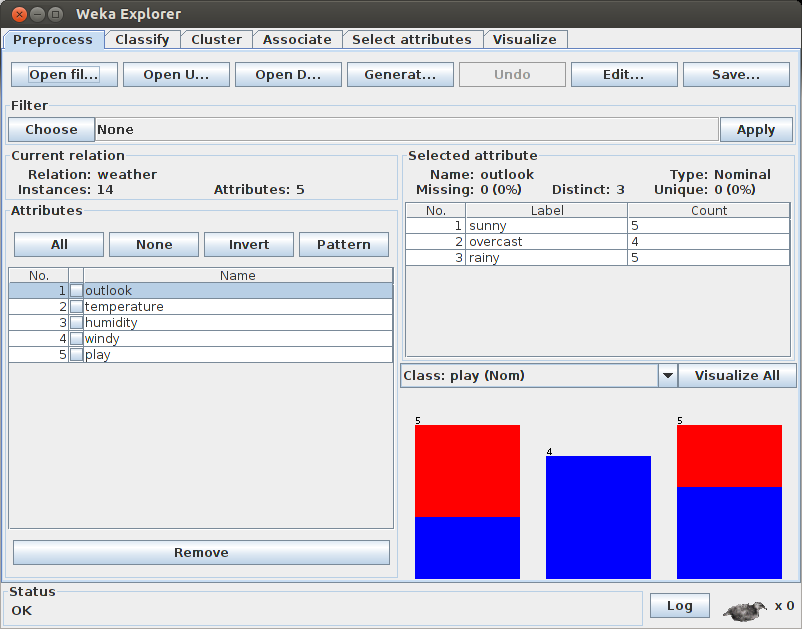
\includegraphics[width=0.75\textwidth]{img/weka.png}
\end{figure}

\subsection{Arquivos ARFF}
\label{sec:prop_arff}

Para que um conjunto de dados possa ser utilizado no WEKA, ele deve estar em um formato específico, denominado ARFF (\emph{Attribute Relationship File Format}, Formato de Arquivo de Relação de Atributos). Um arquivo nesse formato é apresentado na listagem \ref{lst:prop_arff}. Esse é o mesmo arquivo apresentado na figura \ref{fig:prop_weka}, onde é mostrada a visualização dos dados pela interface gráfica.

\vspace{1cm}
\begin{lstlisting}[caption=Exemplo de arquivo no formato ARFF, label=lst:prop_arff]
    @relation weather

    @attribute outlook {sunny, overcast, rainy}
    @attribute temperature real
    @attribute humidity real
    @attribute windy {TRUE, FALSE}
    @attribute play {yes, no}

    @data
    sunny,85,85,FALSE,no
    sunny,80,90,TRUE,no
    overcast,83,86,FALSE,yes
    rainy,70,96,FALSE,yes
    rainy,68,80,FALSE,yes
    rainy,65,70,TRUE,no
    overcast,64,65,TRUE,yes
    sunny,72,95,FALSE,no
    sunny,69,70,FALSE,yes
    rainy,75,80,FALSE,yes
    sunny,75,70,TRUE,yes
    overcast,72,90,TRUE,yes
    overcast,81,75,FALSE,yes
    rainy,71,91,TRUE,no
\end{lstlisting}
\vspace{1cm}

Um arquivo ARFF é um arquivo de texto simples, em um formato padronizado, que combina a descrição dos dados e os dados em si \cite{Hall2009}. Ele é dividido em duas seções. A primeira, chamada de cabeçalho (\emph{header}) contém o nome do conjunto de dados (\emph{@relation}) e a lista de atributos (colunas) e seus tipos (\emph{@attribute}). Esses arquivos também podem conter comentários, que são ignorados quando o arquivo é analisado, e podem ser utilizados para adicionar informações ao arquivo como fonte, licença, etc. Um comentário é inserido através do caractere '\%', e tem efeito até o caractere de nova linha. Após o cabeçalho, vem a seção que contém os dados em si (\emph{@data}).

O nome do conjunto de dados é uma \emph{string} arbitrária, e serve apenas para a identificação na interface (figura \ref{fig:prop_weka}). A lista de atributos é uma sequência de entradas \emph{@attribute}. Cada atributo no conjunto de dados tem uma entrada \emph{@attribute} correspondente, que identifica o atributo. A ordem da declaração deve ser exatamente a ordem em que os atributos são listados na seção de dados. Isso facilita a listagem de dados, onde não é necessário indicar, para cada valor, o atributo ao qual ele se refere. O formato de cada \emph{@attribute} é:

\begin{lstlisting}[caption=Formato de uma entrada \emph{@attribute}, label=lst:prop_attribute_out]
@attribute nome tipo
\end{lstlisting}

O WEKA suporta quatro tipos de atributos. O formato ARFF, no entanto, suporta seis, e a conversão é feita automaticamente:

\begin{description}
    \item[numeric] um atributo que pode ser tanto um número inteiro como real.
    \item[inteiro] tratado pelo WEKA como \emph{numeric}.
    \item[real] tratado pelo WEKA como \emph{numeric}.
    \item[nominal] um atributo com valores pré-definidos. Esses valores são especificados através de uma lista no formato: \{ valor1, valor2, valor3, \emph{...} \}.
    \item[string] uma \emph{string} de caracteres.
    \item[date] uma data, com um campo opcional que especifica o formato da data, como "yyyy-MM-dd HH:mm:ss".
\end{description}

A seção de dados inicia com a entrada \emph{@data}, e segue até o final do arquivo. Nela são listados os valores do conjunto de dados. Cada entrada é representada em uma linha, ou seja, as entradas são separadas pelo caractere de nova linha. Em cada entrada, seus atributos são listados em uma lista separada por vírgulas. Como dito anteriormente, os atributos são identificados pela ordem ordem de declaração, logo ela deve ser a mesma no cabeçalho e nessa seção. Valores ausentes são representados por um caractere de ponto de interrogação (\emph{?}). Os atributos do tipo nominal e \emph{string} são \emph{case sensitive}, e devem ser envolvidos em aspas se contém espaços.

\subsection{Resultados}
\label{sec:prop_results}

A listagem \ref{lst:prop_weka_out} mostra um exemplo dos dados de saída após a execução de um teste de um dos algoritmos (LVQ) em um conjunto de dados de teste. O atributo ``\emph{Scheme}'' mostra o classificador e todos os parâmetros correspondentes utilizados no treinamento. Os atributos ``\emph{Relation}'', ``\emph{Instances}'' e ``\emph{Atttributes}'' mostram informações do conjunto de dados: o nome, número de instâncias e atributos, respectivamente.

Por fim, ``\emph{Test mode}'' mostra o método utilizado para a execução dos testes. As quatro opções disponíveis são:

\begin{description}
    \item[Use training set] Executa os testes utilizando os mesmos dados utilizados no treinamento.
    \item[Supplied test set] Executa os testes utilizando um arquivo de testes fornecido.
    \item[Cross-validation] Executa os testes utilizando \emph{\emph{k}-fold cross-validation} (seção \ref{sec:eval_cross_validation}). O número de \emph{folds} pode ser definido.
    \item[Percentage split] Executa os testes utilizando uma parte dos dados para testes e outra para o treinamento. A procentagem pode ser definida.
\end{description}

A seguir são mostrados dados sobre o processo de treinamento: tempos de execução e informações sobre o modelo gerado pelo classificador. A próxima seção mostra os resultados dos testes. Os dados dessa seção são: número de instâncias corretamente classificadas, número de instâncias incorretamente classificadas, o coeficiente \emph{kappa}, o erro de aproximação e a raiz quadrada do erro de aproximação, o erro relativo e a raiz quadrada do erro relativo e o número total de instâncias.

Também é gerada uma tabela com os resultados para cada classe presente nos dados: taxa de verdadeiros e falsos positivos, \emph{precision}, \emph{recall} e \emph{f-measure} e a área sob a curva ROC.

A última parte é uma matriz de confusão. As colunas dessa matriz mostram a classificação das instâncias e as linhas, a classe verdadeira. Dessa forma, é possível identificar o número de instâncias correta e incorretamente classificadas. Para um conjunto de dados que contém apenas duas classes, essa tabela também mostra o número de falsos positivos e negativos.

\vspace{1cm}
\begin{lstlisting}[caption=Exemplo de saída de uma execução do WEKA, label=lst:prop_weka_out]
    === Run information ===

    Scheme:       weka.classifiers.neural.lvq.MultipassLvq -A
    "weka.classifiers.neural.lvq.Olvq1 -M 1 -C 20 -I 1000 -L 1 -R 0.3 -S 1 -G
    false" -B "weka.classifiers.neural.lvq.Lvq3 -M 1 -C 20 -I 10000 -L 1 -R 0.05 -S
    1 -G false -W 0.3 -E 0.1"
    Relation:     weather
    Instances:    14
    Attributes:   5
                  outlook
                  temperature
                  humidity
                  windy
                  play
    Test mode:    10-fold cross-validation

    === Classifier model (full training set) ===

    -- Training Time Breakdown --
    Pass 0: 17ms
    Pass 1: 51ms
    Total Model Preparation Time: 68ms

    -- Cass Distribution --
    yes :  15 (75%)
    no :  5 (25%)



    Time taken to build model: 0.07 seconds

    === Stratified cross-validation ===
    === Summary ===

    Correctly Classified Instances           5               35.7143 %
    Incorrectly Classified Instances         9               64.2857 %
    Kappa statistic                         -0.4651
    Mean absolute error                      0.6429
    Root mean squared error                  0.8018
    Relative absolute error                  135      %
    Root relative squared error              162.5137 %
    Total Number of Instances                14

    === Detailed Accuracy By Class ===

    Class          TP Rate   FP Rate   Precision   Recall  F-Measure   ROC Area

    yes              0.556     1          0.5       0.556     0.526      0.278

    no               0         0.444      0         0         0          0.278

    Weighted Avg.    0.357     0.802      0.321     0.357     0.338      0.278

    === Confusion Matrix ===

     a b   <-- classified as
     5 4 | a = yes
     5 0 | b = no
\end{lstlisting}

\section{Método de pesquisa}

As atividades da segunda etapa do Trabalho de Conclusão de Curso serão desenvolvidas conforme apresentadas na tabela \ref{tab:prop_cron} e serão descritas à seguir.

A etapa de coleta e preparação de dados envolverá a adaptação dos dados nos conjuntos ao formato de entrada esperado pelo WEKA, já que eles se encontram em estado bruto. O formato mais comum para utilização nesse programa são arquivos \emph{Attribute Relationship File Format} (ARFF, Formato de Arquivo de Atributo-Relação). Um arquivo nesse formato é apresentado na listagem \ref{lst:prop_arff}. Esse mesmo arquivo foi apresentado na figura \ref{fig:prop_weka}, mostrando a visualização pela interface do WEKA.

\vspace{1cm}
\begin{lstlisting}[caption=Exemplo de arquivo no formato ARFF, label=lst:prop_arff]
    @relation weather

    @attribute outlook {sunny, overcast, rainy}
    @attribute temperature real
    @attribute humidity real
    @attribute windy {TRUE, FALSE}
    @attribute play {yes, no}

    @data
    sunny,85,85,FALSE,no
    sunny,80,90,TRUE,no
    overcast,83,86,FALSE,yes
    rainy,70,96,FALSE,yes
    rainy,68,80,FALSE,yes
    rainy,65,70,TRUE,no
    overcast,64,65,TRUE,yes
    sunny,72,95,FALSE,no
    sunny,69,70,FALSE,yes
    rainy,75,80,FALSE,yes
    sunny,75,70,TRUE,yes
    overcast,72,90,TRUE,yes
    overcast,81,75,FALSE,yes
    rainy,71,91,TRUE,no
\end{lstlisting}
\vspace{1cm}

Ainda, podem ser necessários ajustes específicos nos dados para que possam servir como entrada para alguns dos algoritmos, caso estes não tenham suporte aos tipos de dados. Com os dados prontos, iniciará a fase de execução dos diferentes algoritmos sobre esses conjuntos de dados. A coleta dos resultados será feita através dos dados de saída, mostrados na listagem \ref{lst:prop_weka_out}. Com os dados prontos, iniciará a fase de execução dos diferentes algoritmos sobre esses conjuntos de dados. A coleta dos resultados será feita através dos dados de saída, mostrados na listagem \ref{lst:prop_weka_out}.

Uma característica positiva da ferramenta WEKA é a possibilidade de alterar parâmetros tanto do algoritmo em si (caso eles ofereçam essa funcionalidade) quanto da execução do teste em si. Assim, pode-se executar diversos testes, variando esses parâmetros, para ao final comparar também essas configurações. A princípio, será definida apenas uma configuração, que será usada para a execução de todos os testes. No entanto, conforme for possível, poderão ser executados testes variando essa configuração, gerando comparação mais diversificadas.

De posse dos resultados dos testes de todos os algoritmos, iniciará a etapa de análise. Os resultados dos algoritmos imunológicos serão comparados com os resultados dos algoritmos tradicionais. Essa comparação envolve diversos níveis: taxas de erros e acertos (conforme apresentado na seção \ref{sec:eval_fraud}), tempos de execução (que inclui tempo de treinamento do algoritmo e o tempo dos testes), utilização de recursos, etc. Para a visualização dos resultados, serão criados elementos visuais, como tabelas e gráficos.

Esse período também inclui a documentação do processo através da redação da monografia e a apresentação ao fim do semestre.

\begin{table}[h]
    \vspace{1cm}
    \caption{Cronograma}
    \centering
    \begin{tabular}{l >{\arraybackslash}m{4cm} >{\centering\arraybackslash}m{7cm} c}
        \multicolumn{2}{c}{Etapa} & Resultado & Data \\
        \hline
        1 & Coleta e preparação dos dados       & Arquivos no formato esperado pelo WEKA & março/2013 \\
        2 & Aplicação dos algoritmos            & Resultados da execução (taxas de acerto, métricas, tempo de execução, listagem \ref{lst:prop_weka_out} & abril/2013 \\
        3 & Comparação e análise dos resultados & Ranking de resultados & maio/2013 \\
        4 & Conclusão e contribuições           & Análise & junho/2013 \\
        5 & Redação e revisão                   & & março-julho/2013 \\
        6 & Apresentação                        & & julho/2013 \\
    \end{tabular}
    \label{tab:prop_cron}
    \vspace{1cm}
\end{table}
